\clearpage
\section{Experiment}
\label{sec:experiment}

We apply our method to the city of Cologne, to retrieve insights about how different modes of transport interact and how they contribute to the accessibility of the city.
As we want to compare different modes of transport, we will calculate the metric multiple times for different scenarios, each with a different combination of modes of transport.

\subsection{Scenarios}
\label{subs:scenarios}

No matter, the mode of transport, we always allow for walking, for two reasons.
First, walking is the most accessible mode of transport, available to almost everyone and without any additional costs.
Second, most other modes of transport require walking at some point, be it to the next bus stop or to the next available bicycle.

The first scenario we consider is our baseline scenario, which only considers walking.
This scenario measures what is possible without any additional infrastructure. 
Distinct from other scenarios, it does not require any additional cost, thus presenting the most basic form of urban mobility.

Building on this, the second scenario we consider is the scenario of only walking. 
We consider this scenario as the benchmark scenario, as we hope to achieve similar (or even better) results with more sustainable modes of transport.
Therefore, we use it to answer the question of how competitive sustainable modes of transport are in comparison to the traditional mode of travel by car. 

Transitioning from the simplest form of mobility, the third scenario, focused on public transport, becomes essential to understand the effectiveness and accessibility of urban transit systems. 
This scenario evaluates how well-connected and time-efficient public transportation networks are, and their role in reducing reliance on personal vehicles. 
It also investigates the impact of public transport on urban mobility and its potential in contributing to a more sustainable urban environment. 
Specifically, it assesses whether public transport is a viable alternative to the personal car and whether it actually offers significant advantages over walking, considering the X-minute city metric.

Next, in the fourth scenario, we shift our focus to the dynamics of bicycle sharing systems. 
This scenario is important for assessing the feasibility and attractiveness of cycling as a primary mode of transportation in urban areas. 
We will directly compare it to the public transport scenario, to understand which sustainable mode of transport is superior.

Finally, the fifth scenario combines public transport and bicycle sharing, offering insights into the synergy between these two modes of transport. 
This integrated approach mirrors a growing trend in urban mobility solutions, where multi-modal transport options are increasingly favored. 
It underscores how this combination can bridge the gaps in accessibility and efficiency found when each mode is used independently. 
This scenario is expected to be the most competitive against cars, offering a comprehensive and sustainable urban transit model that could reshape the landscape of city mobility.

We summarize the scenarios in Table \ref{table:scenarios}.

\begin{table}[h]
\centering
\begin{tabular}{|p{4cm}|p{5cm}|p{4cm}|}
\hline
\textbf{Scenario} & \textbf{Modules} & \textbf{Key Points} \\
\hline
Walking & Walking & Baseline scenario \\
\hline
Personal Car & Personal Vehicle, Walking & Benchmark scenario \\
\hline
Public Transport & Public Transport, Walking & Evaluate the effectiveness public transport systems \\
\hline
Bicycle Sharing & Vehicle Sharing, Walking & Evaluate the effectiveness of bicycle sharing systems \\
\hline
Public Transport and Bicycle Sharing & Public Transport, Bicycle Sharing, Walking & Evaluate the effectiveness of sustainable multi-modal transport systems \\
\hline
\end{tabular}
\caption{Scenarios for Urban Mobility Analysis}
\label{table:scenarios}
\end{table}

The specific configuration of the module matrices for each scenario can be found in Appendix \ref{app:experiment_module_matrix_configuration}.

\subsection{Data}
\label{subs:data}

To calculate the Pareto sets of the X-minute city metric for the different scenarios, we use four different datasets.
First, we require data that depicts the street network of the city of Cologne.
Second, we need to know the locations of the POIs, which we want to reach.
Third, we need to know the locations of the public transport stops, as well as, the schedules of the public transport.
For the bicycle sharing scenario, we also need to know the locations of the bicycles.
Lastly, we also use land use data to identify where residential areas are located, so that we can calculate the X-minute city metric only for these areas.

As we will query spatial datasets of various formats, from different sources, the area covered by the datasets will not be the same.
Therefore, we first define an area of interest and later trim the datasets to this area.
In our case, this area is defined as the area of the administrative district of Cologne, specifically the "Stadtkreis Köln".
We retrieve the specific boundary of this area with the help of the Overpass API \shortcite{OverpassAPIOverpass}.
The specific query can be found in Appendix \ref{app:overpass_query} and the resulting region can be seen in Figure \ref{fig:area_plus_buffer}.

\begin{figure}
  \begin{center}
    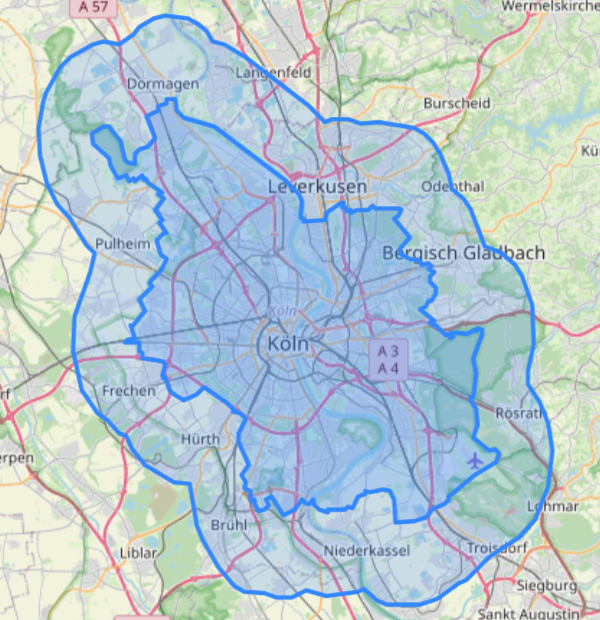
\includegraphics[width=0.55\textwidth]{Figures/experiment/area_plus_buffer.png}
  \end{center}
  \caption{Area of Interest and Buffer Region}\label{fig:area_plus_buffer}
\end{figure}

Additionally, the Figure also shows a buffer region around our area of interest.
This larger region adds a buffer of approximately 5 km and is used by some in parts of our data processing.


\subsubsection{Street Network \& POIs}
\label{subs:street_network_pois}

For the street network and the POIs, we use data from OpenStreetMap (OSM) \shortcite{OpenStreetMap}.
To use OSM data in practice various tools and services have been developed.
Among these we use, pyrosm \shortcite{Pyrosm} which is a Python library designed specifically for reading OSM data in different formats and conducting data processing operations.
Through pyrosm, we can automatically fetch data from sources like Geofabrik \cite{GeofabrikDownloadServer} and BBBike \cite{BBBikeExtractsOpenStreetMap}, which are two of the most popular OSM data providers.
In our case, we use the data for the city of Cologne from BBBike.
However, due to the flexibility of pyrosm, it is easily possible to use data from other sources as well and expand our analysis to other cities.

After retrieving the data, we retrieve a graph representation of the street network trimmed to the buffered area of interest.
Using the buffered region is important, because without it calculating the X-minute city metric at the border of the area of interest would result in a higher value than the actual value.
As a last cleaning step, we remove all nodes, that are not part of the largest weakly connected component.
A weakly connected component is a subgraph in which, if all directed edges were treated as undirected, any two vertices from the subgraph would be connected.
Multiple weakly connected components in graphs derived from OSM data, mostly happen at the border of the considered area and can be neglected.

Because we consider multiple different modes of transport on the network, it is important to filter out all edges that are not accessible by the respective mode of transport.
To do so, we use pyrosm's built-in filtering functionality.
For reproducibility, we list the filters that pyrosm uses in Appendix \ref{app:pyrosm_network_filter}.

To retrieve the POIs, we use the Overpass API \shortcite{OverpassAPIOverpass}.
We retrieve all POIs that fall into one of our predefined categories specified in Section \ref{subsec:metric} inside the area of interest plus the buffer mentioned before.

\subsubsection{Public Transport}
\label{subs:public_transport}

To handle public transport data, we use the General Transit Feed Specification (GTFS) \shortcite{GTFS}.
To retrieve it we rely on the Mobility Database \shortcite{MobilityDatabase}.
This database serves as an open-source repository containing links to publicly available GTFS feeds globally, standing as the subsequent version of TransitFeeds \shortcite{OpenMobilityDataPublicTransit}.
Similarly to the OSM data, we trim the GTFS data to the area of interest plus the buffer.
The GTFS data is also cleaned and converted into a format that is more suitable for our algorithm, or more specifically McRAPTOR, which is part of our algorithm.
Specifically, there are two major incompatibilities between the GTFS specification and RAPTOR's notion of routes and trips.
Firstly, each trip belonging to a single route in RAPTOR visits the same stops in the same order.
It is not possible that a trip skips some stops that another trip of the same route visits, much less use a completely different sequence of routes.
In GTFS routes do allow that, as they are much more a group of trips that is presented to the rider under the same name or identifier.
Secondly, GTFS trips allow visiting the same stop multiple times, which is not allowed in RAPTOR.
To overcome these difference we split up routes into smaller routes, that follow the same sequence of stops.
Additionally, e also remove circular trips, altogether.


\subsubsection{Bicycle Sharing}
\label{subs:bicycle_sharing}

Our bicycle sharing data was retrieved from the NextBike API over a time period of one year.
The data consists of all trips that were made with the NextBike system in the city of Cologne from the 15th of January 2022 to the 31st of August 2023.
To get representative samples of the locations of all bicycles we employ the following strategy.
We first discretize the data spatially and temporally.
For the temporal discretization, we derive the location of each bicycle every hour.
For the spatial discretization, we use H3 hexagons with a resolution of 9.
The resulting data is the information how many bicycles were at each hexagon at each hour.
This data is then used as an input for k-medoids clustering \shortcite{rdusseeun1987clustering} with a k of 4.
K-medoids, also known as PAM (Partitioning Around Medoids) algorithm, is a clustering technique that partitions a dataset into K clusters, where each is assigned a medoid, that is the most centrally located object in a cluster. 
Unlike K-means, which uses mean values as cluster centers, K-medoids an actual data point as the center of a cluster.
This has the advantage that the centers are part of the dataset and therefore are realistic samples.
We use the resulting medoids as different configurations of the locations of the bicycles.

\subsubsection{Land Use}
\label{subs:land_use}

To identify the residential areas, we use the land use data from the CORINE Land Cover (CLC) project \shortcite{CORINELandCover}.
The data covers the whole of Europe and is publicly available, which again makes it possible to expand our analysis to other cities in Europe.
We trimmed the data to the area of interest and then filtered for the land use types "Continuous Urban Fabric" and "Discontinuous Urban Fabric".
These two land use types represent the residential areas of the city.
The residential areas inside the area of interest are shown in Figure \ref{fig:input_hexagons_residential_areas}.
Additionally, the Figure shows the hexagons of resolution 9 that are found inside the residential areas.

\begin{figure}
  \begin{center}
    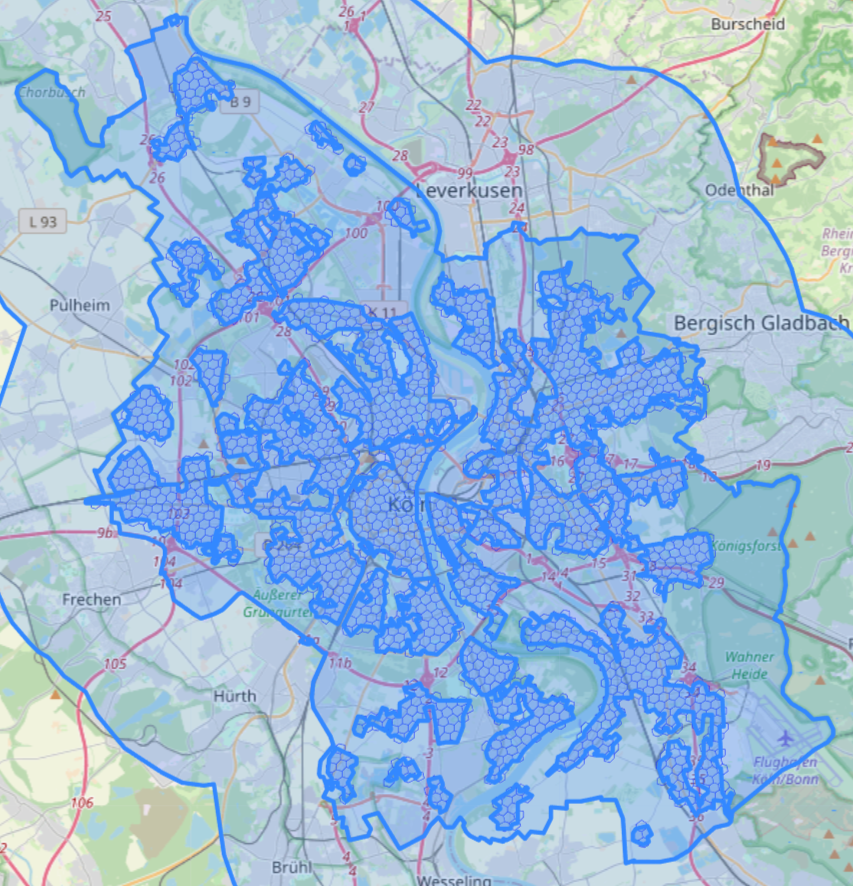
\includegraphics[width=0.65\textwidth]{Figures/experiment/input_hexagons_residential_areas.png}
  \end{center}
  \caption{Area of Interest and Buffer Region with Residential Areas and Input Hexagons}
  \label{fig:input_hexagons_residential_areas}
\end{figure}


\subsection{Assumptions}
\label{subs:assumptions}

To calculate the X-minute city metric we have to abstract from reality to some degree.
We do so by making the following plausible assumptions.

Firstly, we assume that travelling along an edge on the street network, by walking, cycling or driving, is always proportional to the length of the edge.
To obtain the time it takes to travel along an edge, we divide the length of the edge by the speed of the mode of transport.
The different speeds for the different modes of transport are listed in Table \ref{table:speeds}.

\begin{table}[h]
\centering
\begin{tabular}{|c|l|}
\hline
\textbf{Mode} & \textbf{Speed (m/s)} \\
\hline
Walking & 1.4 \\
\hline
Cycling & 4.0 \\
\hline
Driving & 11.0 \\
\hline
\end{tabular}
\caption{Speeds for Different Modes of Transport}
\label{table:speeds}
\end{table}

The walking speed is consistent with the measurement that \cite{willberg15minuteCityAll2023} made in their study.

We also pose some assumption on the transitioning between different modes of transport, as well as, in the case of public transport, the transfer time at the stops.
For the transfer time at stops we assume a fixed time of one minute.
To transition from any OSM network-based mode of transport to public transport, we assume that the stop is precisely at the location the closest node of the OSM network.
As OSM networks contain public transport stops, there should be no difference between the two.
Similarly, we assume that the bicycles are located at the closest node of the OSM network.
As the OSM network, especially in city is very dense, this assumption is reasonable.
We also assume that bicycles and cars can be parked anywhere on their respective network for the sake of simplicity.


\subsubsection{Pricing}
\label{subs:pricing}

We try to implement a pricing scheme in our scenarios that represents the real-world circumstances as closely as possible.

For bicycle sharing, we use the pricing scheme of NextBike, which is 1€ every 15 minutes.
To depict this we add a hidden value to the labels processed in MLC that depicts how long the current bicycle trip is.
As two consecutive bicycle trips are considered separately we nullify this hidden value after each run of MLC.

For public transport, we use the pricing scheme of the Cologne Transport Authority (KVB), which is 2.20€ for trips that span four stops or less.
For any trip that spans more than four stops or any multitude of trips the KVB charges 3.20€.
To depict this we add a hidden values to the labels processed in McRAPTOR that depicts how many stops the traveler already traversed.
Because two consecutive trips are considered together, we don't need to nullify the hidden value.

% TODO: personal car
